\documentclass[12pt,t]{beamer}

\beamertemplatenavigationsymbolsempty

% usepackage
%\usepackage{template/dbt}
\usepackage{listings,graphics}

\definecolor{comments}{RGB}{81,81,81}
\definecolor{keywords}{RGB}{255,0,90}

% lstlisting
\lstset{
    language=C,
    basicstyle=\footnotesize\ttfamily,
    keywordstyle=\color{keywords},
    showspaces=false,
    showstringspaces=false,
    commentstyle=\color{blue}\emph
    %frame=single,
    %rulecolor=\color{comments},
    %rulesepcolor=\color{comments},
    %backgroundcolor = \color{lightgray}
}

\usetheme{default}

\usepackage[
    type={CC},
    modifier={by-nc-nd},
    version={4.0},
]{doclicense} 

\newcommand{\courseurl}[0]{https://www.cct.lsu.edu/\string~pdiehl/teaching/2021/4997/}
\newcommand{\coursetimeline}[0]{https://www.cct.lsu.edu/~pdiehl/teaching/2021/4997/timeline.pdf}
\newcommand{\coursesyllabus}[0]{https://www.cct.lsu.edu/~pdiehl/teaching/2021/4997/syllabus.pdf}
\newcommand{\coursename}[0]{Math 4997-3}
\newcommand{\coursemailinglist}[0]{https://mail.cct.lsu.edu/mailman/listinfo/par4997}
\newcommand{\coursesemester}{Fall 2021}








% frame slide
\title{\coursename}
\subtitle{Lecture 4: N-Body simulations, Structs, Classes, and generic functions}

%\author{\href{}{}}
%\institute {
%    \href{}{\tt \scriptsize \today}
%}
\date {
 \tiny \url{https://www.cct.lsu.edu/~pdiehl/teaching/2019/4977/}
\vspace{2cm}
\doclicenseThis  
  
}



\usepackage{ifxetex}

\ifxetex
\usepackage{fontspec}
\setmainfont{Raleway}
\fi

\begin{document} {
    \setbeamertemplate{footline}{}
    \frame {
        \titlepage
    }
}

\frame{

\tableofcontents

}

\AtBeginSection[]{
  \begin{frame}
  \vfill
  \centering
  \begin{beamercolorbox}[sep=8pt,center,shadow=true,rounded=true]{title}
    \usebeamerfont{title}\insertsectionhead\par%
  \end{beamercolorbox}
  \vfill
  \end{frame}
}


\begin{frame}{$N$-body simulations\footnote{\tiny By Michael L. Umbricht - Own work, CC BY-SA 4.0}}

\begin{figure}
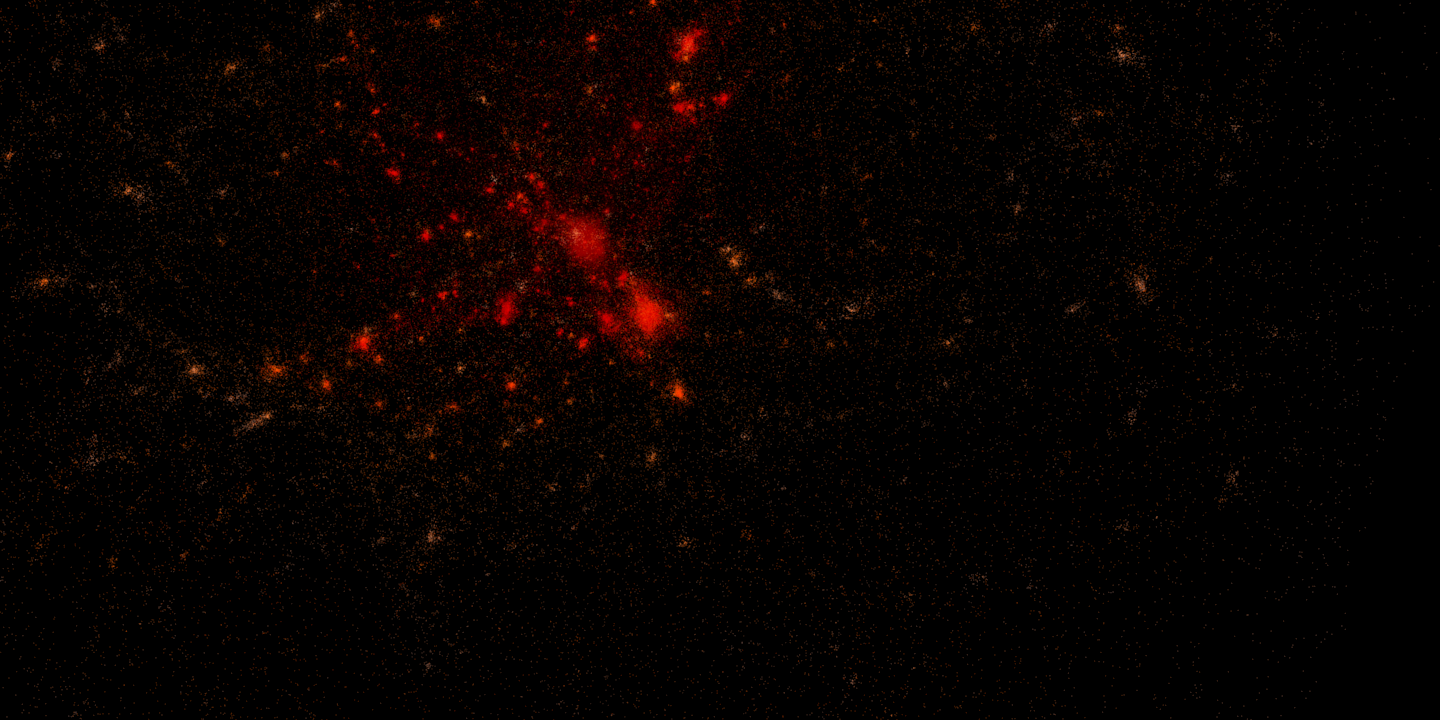
\includegraphics[width=0.5\linewidth]{./images/Galaxy_cluster_sim.png}
\end{figure}


The $N$-body problem is the physically problem of predicting the individual motions of a group of celestial objects interacting with each other gravitationally.

\begin{block}{Informal description:}
Predict the interactive forces and true orbital motions for all future times of a group of celestial bodies. We assume that we have their quasi-steady orbital properties, e.g.\ instantaneous position, velocity and time.
\end{block}

\end{frame}



\end{document}